\section{Overview of SeqStar}\label{sec:framework}
We demonstrate the workflow of SeqStar in this section,
and use an example to show the query processing stages.
\subsection{SeqStar Workflow}
\begin{figure}[ht]
  \centering
  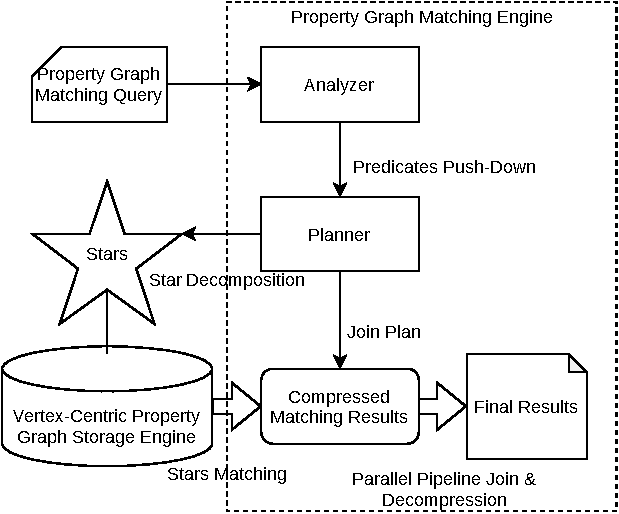
\includegraphics[width=0.48\textwidth]{img/architecture.pdf}
  \caption{SeqStar workflow.}\label{img:architecture}
\end{figure}
Figure~\ref{img:architecture} shows the workflow of SeqStar. There are mainly two building blocks in SeqStar: the storage engine and the property graph matching engine.
Both are specially designed to deal with the property graph matching problem efficiently.

Traditional graph storage engines such as used in graph databases store the in-edges and out-edges separately for each vertex.
Because of the complexity in property graphs,
such a storage method is not suitable and would incur many unnecessary random disk accesses.
We develop a vertex-centric property storage model to store all information related to one vertex together to address the problem (\S\ref{sec:storage}).


Based on the storage model,
we propose an efficient property graph matching engine that is able to execute real-world complex queries (\S\ref{sec:match}).
The core of the graph matching engine is the planner, which  decomposes the pattern into a series of stars.
Compared with existing works, we take a step further by introducing
(1) a matching result compression algorithm which reduces the cost of materializing intermediate results,
(2) a predicate pushdown optimizer that is able to filter out unnecessary matchings in early stages and mitigate the burden of the join process.
\subsection{Query Processing Stages}
Here is an example of how a concrete query gets executed in SeqStar.
Consider the Cypher (Neo4j's graph query language) query in Figure~\ref{img:cypher_query},
which generates the pattern graph in Figure~\ref{img:running_example} (b):

\begin{figure}[ht]
  \begin{Verbatim}[fontsize=\small]
    MATCH (u1:Person)-[:FOLLOWS]->(u2:Person)-[:FOLLOWS]->(u1),
          (u1)-[:FOLLOWS]->(u3:Person)-[:FOLLOWS]->(u1),
          (u1)-[:REPOSTS]->(u4:Media),
          (u2)-[:LIKES]->(u4)<-[:LIKES]-(u3)
    WHERE u2 > u1 AND NOT (u3 <= u1 OR u4 >= 8)
  \end{Verbatim}
  \caption{Example query.}\label{img:cypher_query}
\end{figure}

\begin{figure*}[ht]
  \centering
  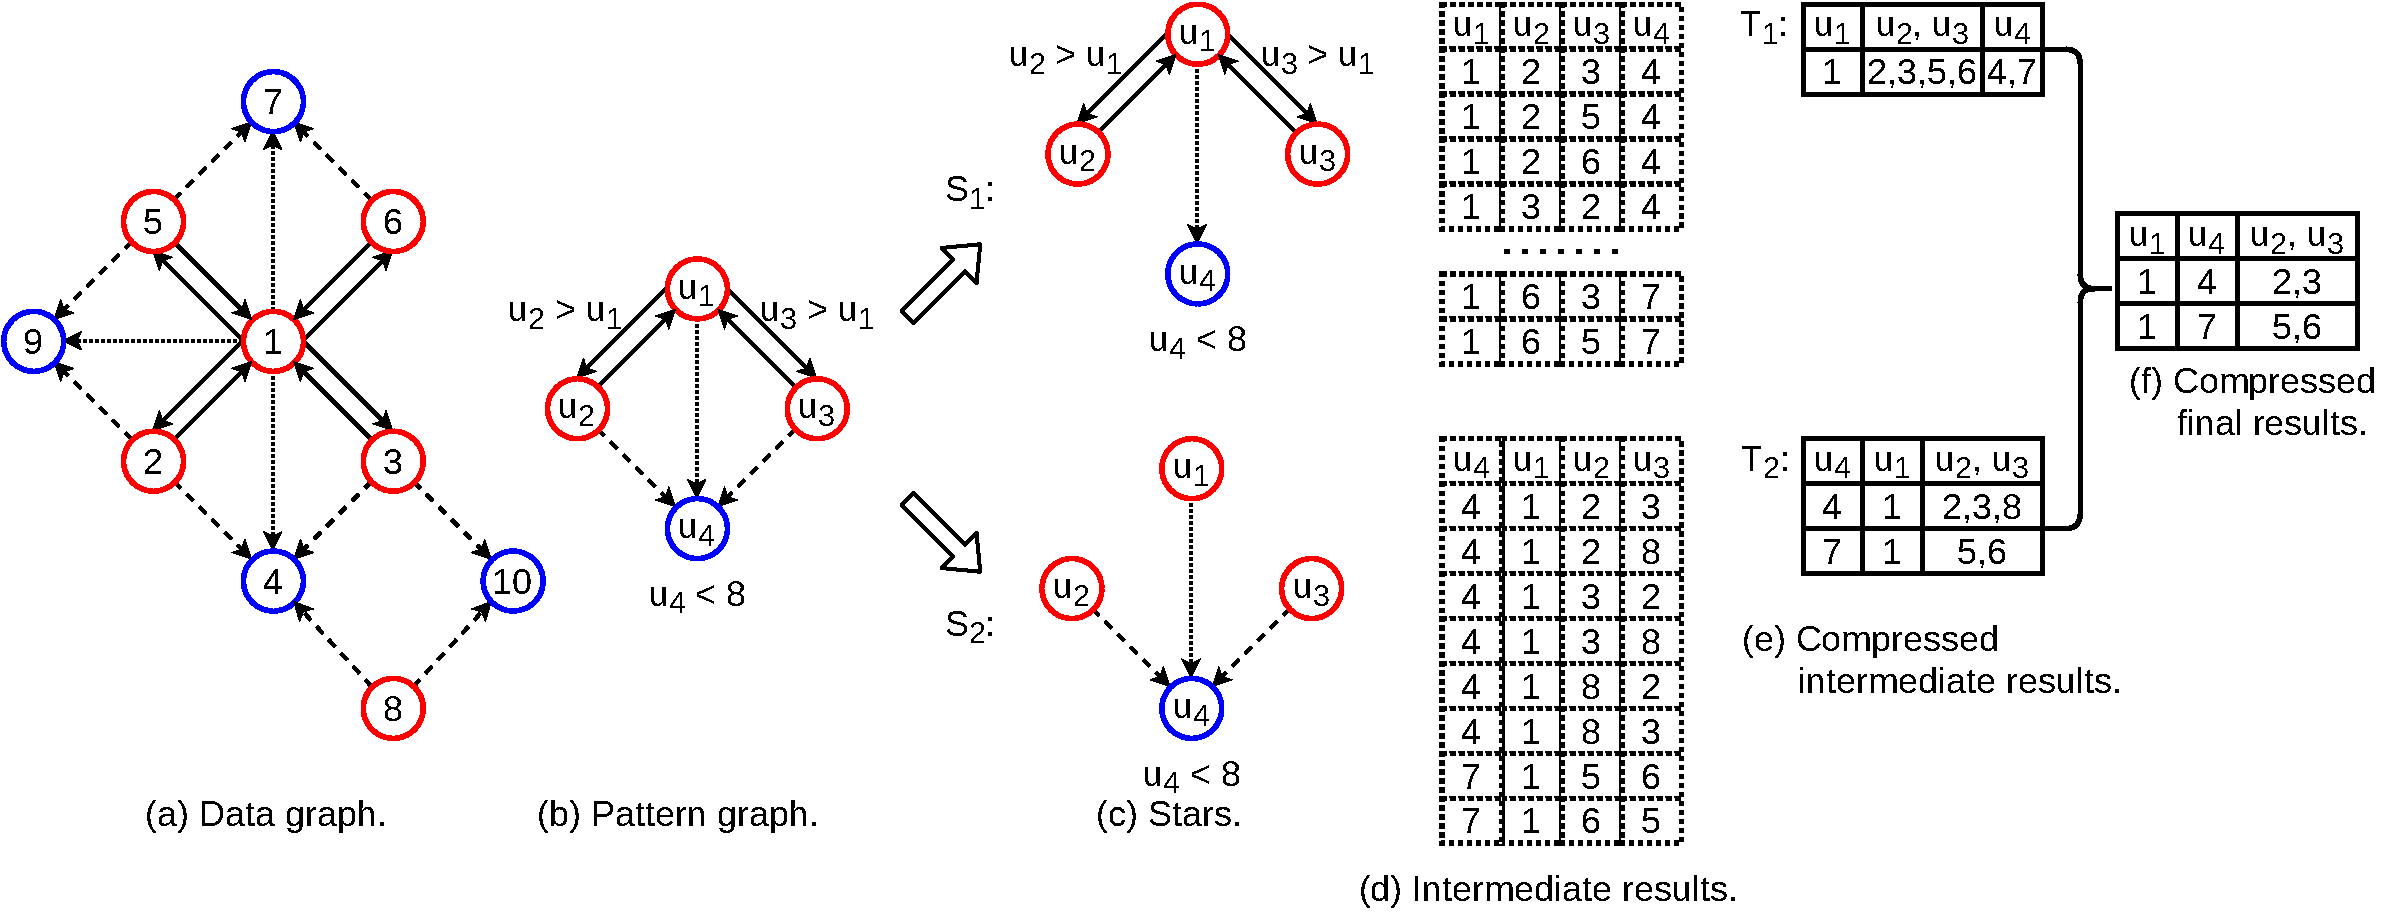
\includegraphics[width=\textwidth]{img/running_example.pdf}
  \caption{Working stages of the example query.}\label{img:running_example}
\end{figure*}

The analyzer firstly analyzes the WHERE clause and extract useful filtering information for early stage filtering.
SeqStar rewrites the WHERE clause to AND-separated expressions `$u_2 > u_1$ AND $u_3 > u_1$ AND $u_4 < 8$' by applying De Morgan's law.
The searching conditions $u_2> u_1$, $u_3 > u_1$ and $u_4 < 8$ are then attached to the pattern graph (Figure~\ref{img:running_example} (b)).
Based on the analysis result and the statistical information of the data graph,
the planner dynamiclly selects a connected vertex cover ($u_1, u_4$) in the pattern as the roots of stars.
The star generating algorithm keeps all the relevant edges and additional searching conditions in order to filter out unnecessary matchings as early as possible.

With the help of SeqStar's vertex-centric storage engine,
all the stars can be matched by only one sequential scan on the data graph (\S\ref{sec:match_star}).
For example, to match star $S_2$,
SeqStar seeks to the vertices labeled with ``Media'' (colored in blue) quickly by searching the index in the storage engine.
The candidate vertices $4, 7, 9, 10$ (vertices are identified by their IDs in integers) may match the root $u_4$.
Then SeqStar scans the candidate vertices sequentially and finds that only vertex $4, 7$ can be matched (vertex $9$ and $10$ violate the constraint $u_4 < 8$).

The intermediate results from star matching are not stored as conventional flat and incarnated rows. Instead, SeqStar compresses the intermediate results and uses pipeline joins without incarnation of some intermediate rows.

SeqStar compresses the intermediate results by digging equivalence classes among vertices and postponing Cartesian product to reduce memory usage (\S\ref{sec:match_compress}).
In the decomposed stars, $u_2$ and $u_3$ have the same label, and they also have the same connections to the root $u_1$ or $u_4$ ($u_2 > u_1$ and $u_3 > u_1$ are equivalent in this case because they both represent the filter $f(x): x > u_1$).
We say that $u_2$ and $u_3$ both belong to the same \emph{neighbor equivalence class}.
For each neighbor equivalence class, the matched vertices are stored together as an \emph{image set}.
For example $\{2, 3, 5, 6\}$ in $T_1$ is the image set of $u_2$ and $u_3$.
An \emph{image set} is the basic structure to hold the intermediate results.
While scanning each vertex $v$ in the data graph,
SeqStar checks the neighbors of $v$ and stores the matched neighbors together as image sets.
To match the star $S_2$,
for each candidate e.g., vertex $4$, SeqStar scans the neighbors of vertex $4$ and finds that $u_1$'s image set is $\{1\}$,
the image set of $u_2, u_3$ is $\{2, 3, 8\}$.
The tuple $(4, \{1\}, \{2, 3, 8\})$ is then appended to the compressed intermediate results, as a \emph{SuperRow}.
Note that the first column contains only one vertex, which matches the root of a star.

Finally, SeqStar performs the joins on SuperRows to obtain the final results (\S\ref{sec:match_join}) without the incarnation of intermediate rows. The planner generates a join order ($T_1 \Join T_2$ in this case) based on the statistical information of the SuperRows.
For each SuperRow $R_1$ in $T_1$, SeqStar scans the image set of $u_4$ and finds the corresponding SuperRow $R_2$ in $T_2$.
The join result of $u_2$, $u_3$ is obtained by the intersection if the corresponding columns of $R_1$ and $R_2$,
i.e., $\{2, 3, 5, 6\} \cap \{2, 3, 8\} = \{2, 3\}$, $\{2, 3, 5, 6\} \cap \{5, 6\} = \{5, 6\}$.
If more than two stars are decomposed from the pattern graph,
instead of join them one by one,
the planner in SeqStar will generate a pipeline plan to multi-join on the SuperRows.
By doing so, no new intermediate rows will be generated.
SeqStar generates the compressed final results in a stream manner.
The decompression by Cartesian product to get the final results is not performed     unless required. The compression and pipeline joining can efficiently reduce the memory consumption during computation.

%and the decompression is done by doing Cartesian production on the fly to report the final answer.

%% The vertex-centric storage engine is designed to be I/O efficient and support the real-world property graph well.
%% The conventional way to store graphs on disk is to store the in/out-edges separately for each vertex,
%% via the compressed sparse column (CSC) and the compressed sparse row (CSR) format~\cite{DBLP:conf/sc/PearceGA10}.
%% However, we find that the conventional graph storing method has limitations for real-world property graph:
%% because of the existence of multi-edges,
%% one has to scan all the in/out-edges to check whether a vertex could be matched if the graph is stored in the traditional way, which is time consuming and I/O inefficient.
%% To address this problem, in Section~\ref{sec:storage},
%% we propose a vertex-centric storage model by storing all the necessary local information together with the neighbors,
%% such that all the unnecessary scanning are avoided.
%% Moreover, we develop two kind of simple indices to boost the searching of vertices, which reduces I/Os even further.

%% The property graph matching engine adopts a join-based method.
%% Generally speaking, there are two kinds of approaches to solve the graph isomorphism problem:
%% one is the tree-based searching algorithm~\cite{DBLP:journals/jacm/Ullmann76,DBLP:conf/sigmod/HanLL13}, and the other is the join-based method~\cite{DBLP:journals/pvldb/LaiQLC15,DBLP:journals/pvldb/QiaoZC17,DBLP:journals/pvldb/MhedhbiS19}.
%% Because of the poor locality of graphs, significant random disk reads may incur when implementing an out-of-core tree-based searching algorithm~\cite{DBLP:conf/sigmod/KimLBHLKJ16}, and thus we choose the join-based approach.
%% The most fundamental problem for a join-based algorithm is to choose the basic matching unit.
%% A straightforward approach is to match the edges of a pattern and then join on the edges' matching results,
%% however, incredible amount of useless intermediate results would be generated by doing so,
%% because an edge contains very little filtering information such as degrees and neighborhood structures.
%% Some authors address the problem by joining on more complex structures such as multi-hop edges or frequent subgraphs,
%% however, it is costly to pre-build proper indices and they require super-linear space~\cite{DBLP:journals/pvldb/SunWWSL12}.
%% Based on these observation, we make a trade-off by choosing stars as our basic unit.
%% Thanks to our vertex-centric storage model, in Section~\ref{sec:match_star}, we'll show that we could scan the huge data graph at most once to obtain the stars' matching results, and all the disk accesses are sequential.
%% Some authors also use star-like structures as their join unit~\cite{DBLP:journals/pvldb/SunWWSL12,DBLP:journals/pvldb/LaiQLC15}, however, we take more steps further by improving the star decomposition algorithm to contain as much filtering information as possible, and our experiment shows that our algorithm could reduce the size of intermediate to $???\%$ and obtain $???\times$ speed-up.

%% For real-world billion node graphs, the intermediate result is another challenge that must be conquered.
%% Even though we could use stars to filter out many unnecessary matchings,
%% the intermediate results could still be gigantic for really huge graphs.
%% Moreover, the intermediate result grows exponentially with respect to the size of the data graph,
%% and they could be even larger than the original data graph.
%% Our experiment shows than a data graph with $???x$ edges may generate $???x$ ($???\times$) rows of matching results.
%% Most of the existing work rely on large physical memory to store the huge intermediate results,
%% which is financially expensive and limit the application of property graph matching.
%% To solve the challenge, in Section~\ref{sec:match_compress}, we design a very compact compression algorithm for stars' matching results.
%% By postponing the Cartesian product and digging the equivalence classes among the vertices in a star,
%% the compression ratio reaches as high as $10^{11}$ (Section~\ref{sec:experiments}).
%% And the compressed data is designed to be written sequentially such that we could write them to disk efficiently when memory is limited, i.e., solving a large property graph matching problem on a laptop.
%% Moreover, in Section~\ref{sec:match_join}, we propose a parallel pipeline join algorithm that is able to join directly on the compressed data.

%% A graph matching query consists two parts: the pattern graph description part (the MATCH clause) and the constraint specification part (the WHERE clause).
%% For example, Figure~\ref{img:cypher_query} shows the Cypher query (Neo4j's graph query language) corresponds to the pattern in Figure~\ref{img:pattern_graph}.
%% Existing graph matching frameworks usually neglect the WHERE clause,
%% because they could always be applied as filters after the graph isomorphism result is obtained.
%% However, the WHERE clause is ubiquitous in real-world property matching queries and they contains many user specified constraints~\cite{DBLP:journals/csur/AnglesABHRV17},
%% it is desirable to push them down to the graph isomorphism searching phase and make full use of these searching constraints.
%% However, it is still challenging to pushdown the predicates, because it depends on the graph matching algorithm and the predicates may involve in vertices among different stars.
%% To address this problem, in Section~\ref{sec:match_optimize}, we propose a novel predicates splitting algorithm that is able to extract useful searching constraints from the WHERE clause and push them down to the star matching process,
%% and reduces the intermediate results further.
%% Our experiment shows that, we could save $???\%$ of the space if the WHERE clause is handled properly,
%% and the overall performance is $???\times$ better then the naive approach.
